\documentclass[12pt]{article}

\usepackage{amsfonts,latexsym,amsthm,amssymb,amsmath,amscd,euscript,mathrsfs}
\usepackage{framed}
\usepackage{fullpage}
\usepackage{graphicx}
\usepackage{fancyhdr}
\usepackage[margin=3cm, headsep=24pt, headheight=2cm]{geometry}
\usepackage [english]{babel}
\usepackage [autostyle, english = american]{csquotes}
\usepackage{verbatim}
 \newcommand{\qpartial}[2]{\dfrac{\partial #1}{\partial #2}}
\pagestyle{fancy}
\fancyhf{}
\rhead{Forrest Flesher and Vinh-Kha Le}
\lhead{Econ 1011a Modeling Project 2}
\rfoot{Page \thepage}


\title{Poetry and Mathematics in Skillistan} 
\author{Forrest Flesher, Vinh-Kha Le}

\begin{document}
\maketitle



Skillistan is a simple economy with only one type of firm that requires two types of workers:
those who can do math (M-types) and those who can write poems about math in addition
to doing math (P-types). The P-types are more productive than M-types. Firms
require some capital investment in the form of toys for the workers to play with while they
work. Residents can always choose to not work and earn a reservation wage pondering the
nature of reality. Note that the residents of Skillistan only derive utility from the wage
they obtain and none from leisure: pondering the nature of reality is no more pleasant
than doing math or writing poetry.

\begin{enumerate} 

	\item{Write down a model for the firm}
	
\begin{enumerate}

	\item{How many M-types and P-types will the firm hire?}
	\item{What will be the wage offered to the M-types and the P-types?}

\end{enumerate}

\section*{Part 1}

	We begin with some basic assumptions and notes on notation:
	
\begin{itemize}

	\item{The firm is profit maximizing, and produces only one good (alternatively, the firm could produce a vector of goods, with a corresponding vector of prices, but we assume one good here to simplify the model)}
	\item{The firm experiences decreasing marginal gains to capital and labor, so as to satisfy sufficient second order conditions for profit maximization}
	\item{The firm cannot set wages or prices}
	\item{The price of capital is fixed at $r$, and the wages of M-types and P-types are $w_m$ and $w_p$ respectively, and the market price of the good produced is $q$}
	\item{We denote the amount of M-types and P-types hired by the firm by $L_m$ and $L_p$ respectively, and the amount of capital as $K$}
	\item{The firm must hire both types of workers to have any production.  This assumption comes from the part of the problem statement that says "the firm \textit{requires} two types of workers"}
	\item{The population is homogeneous - all people have the same utility function.  This is because in the problem statement, it is noted that residents derive utility only from wages (and thus not from any amenities of the job).  If two people have a different utility function, we can monotonically transform one to the other, since people will always prefer more money to less.}
\end{itemize}

Given these assumptions, note that the firm has a production function $f(K,L_m,L_p)$.  Given this and the other exogeneous variables, we have that the firm will obtain profit of $q f(K,L_m,L_p) - w_m L_m - w_p L_p - rK$.  We assumed that the production function satisfies relevant second order conditions, so we have that the following first order conditions are sufficient to characterize a maximum:
\begin{align*}
q f_K(K, L_m, L_p) &= r \\
q f_{L_m}(K, L_m, L_p) &= w_m \\
q f_{L_p}(K, L_m, L_p) &= w_p \\
\end{align*}

Dividing the above equations by each other gives that the following must hold (with arguments suppressed):
\begin{align*}
f_{L_m} w_p &= f_{L_p} w_m \\
f_{L_m} r &= f_K w_m \\
f_{L_p} r &= f_k w_p \\
\end{align*}

Now, we know that P-types are more productive that M-types, which implies that $f_{L_p} > f_{L_m}$, for equal values of $L_p$ and $L_m$.  From the above equations, we have the ratio $\dfrac{f_{L_m}}{f_{L_p}} = \dfrac{w_m}{w_p}$.  Thus, we see that if the wages are equal, then we have $f_{L_p}(K,L_m,L_p) = f_{L_m}(K,L_m,L_p)$.  This means that if the wages are equal, the firm will hire more P-types, and fewer M-types.  Similarly, if the wages for P-types are lower than M-types, then the firm will definitely hire more P-types.  If the wage of M-types is lower than the wage of P-types, then it is not certain whether the firm will hire more M-types or P-types.  However, they will still hire where $\dfrac{f_{L_m}}{f_{L_p}} = \dfrac{w_m}{w_p}$.  We see that the wage of the P-types versus M-types depends on the difference in productivity - the more productive the P-type relative to the M-type, the higher the difference in wages.  This is not necessarily obvious now, since we assume the firm takes wages and prices as exogeneous, but it will be discussed in more detail later, in discussion of market equilibrium.  

Now, we know that P-types are more productive that M-types, which implies that $f_{L_p} > f_{L_m}$, for equal values of $L_p$ and $L_m$.  From the above equations, we have the ratio $\dfrac{f_{L_m}}{f_{L_p}} = \dfrac{w_m}{w_p}$.  Thus, we see that if the wages are equal, then we have $f_{L_p}(K,L_m,L_p) = f_{L_m}(K,L_m,L_p)$.  This means that if the wages are equal, the firm will hire more P-types, and fewer M-types.  Similarly, if the wages for P-types are lower than M-types, then the firm will definitely hire more P-types.  If the wage of M-types is lower than the wage of P-types, then it is not certain whether the firm will hire more M-types or P-types.  However, they will still hire where $\dfrac{f_{L_m}}{f_{L_p}} = \dfrac{w_m}{w_p}$.  We see that the wage/number of the P-types versus M-types depends on the difference in productivity.  The actual wages that must be offered are discuessed below. 

Now, to better understand the relationships between wages and labor, we consider some comparative statics.  For brevity, and because the equations are symmetric, we take comparative statics of $L_p$ and $L_m$ with respect to $w_m$ (the results with respect to $w_p$ are analogous):
$$
  \qpartial{L_p}{w_m} = \frac{f_{K L_m} f_{L_p L_p} - f_{K L_p} f_{L_m L_p}}{q \left(f_{K K}
   \left(f_{L_m L_p}^2-f_{L_m L_m} f_{L_p L_p} \right) + f_{K L_m} ^2 f_{L_p L_p}-2
   f_{K L_m} f_{K L_p} f_{L_m L_p} + f_{K L_p}^2 f_{L_m L_m}\right)}
$$
$$
	\qpartial{L_m}{w_m} = \frac{f_{K L_p}^2-f_{KK} f_{L_p L_p}}{q \left(f_{KK}
   \left(f_{L_m L_p}^2-f_{L_m L_m} f_{L_p L_p}\right)+f_{K L_m}^2 f_{L_p L_p}-2
   f_{K L_m} f_{K L_p} f_{L_m L_p}+f_{K L_p}^2 f_{L_m L_m}\right)}
$$
The denominator is the same in both expressions above, and is always positive.  Thus, we see that since $f_{K L_p}^2-f_{KK} f_{L_p L_p} < 0$, we have that $\qpartial{L_m}{w_m}$ is always negative, meaning an increase in the wages of M-types will always cause a decrease in the wages of M-types.  The other equation has an ambiguous sign.  However, since we know that P-types can also do math, the job of M-types, we can assume that these jobs are substitutes, and thus we have that $f_{K L_m} f_{L_p L_p} - f_{K L_p} f_{L_m L_p} > 0$, so that $\qpartial{L_p}{w_m}$.  Thus, an increase in the wage of the M-types will cause an increase in the number of P-types hired, and by symmetry, vice-versa.  In the case of constant returns to scale, these comparative statics are ambiguous.  

In this first part, we can assume that any person can change freely between being a P-type and an M-type without barrier (which will not always be true, as we see in the next part). We then have that the wages of P-types and M-types must be equal, since otherwise the utility to being one would be greater than that of the other, so that there would only be one type of worker.  When there is only one type of worker, the firm is not profit maximizing, so it must increase the wages of the other type until the two are equal.  Thus, we see that $f_{L_p} = f_{L_m}$.  This implies that the firm will hire more P-types than M-types.  Note, also in this case, the wage offered to the P-types and M-types must be the same as or greater than the reservation wage - otherwise everyone would choose to work, and the equilibrium would shift the wages back up so that people will work.  In fact, the wages must be \textit{equal} to the reservation wage, since otherwise the firm could just cut the wages to increase profit, and no one would switch and choose to be unemployed.  Thus, we have that in equilibrium, the wages of all of these will be the same, and there will be more P-types than M-types employed by the firm, and some number (possibly zero) unemployed people.   
 

	\item{All residents graduate from Skillistan High where they learn how to do math without
paying any fees. When they graduate from high school, all residents of Skillistan are
identical M-types. Afterwards, they can choose to attend Skillvard College where
they can learn how to write poems about math and become P-types but they have
to pay tuition fees.}

\begin{enumerate}

	\item{Derive a condition in terms of the wages in equilibrium for M-types and P-types
and in terms of the cost of Skillvard high for when M-types will choose to become
P-types.}

\end{enumerate}

\section*{Part 2}

We consider a two period case: the first period is the time that it takes for a person to go through college, and the second is the rest of the time they are alive.  Each person will maximize sum of their utilities in each period , with a discounting factor on the second period, which is less than one, assuming people value money more in the current period.  That is, people maximize $U_{P_1} + \beta U_{P_1}$, where $U_{P_1}$ is the utility in the first period and $U_{P_2}$ is the utility in the second period.  Assume that people spend all money during each period (so that there are no savings, and utility is just the amount of money they have in that period).  Additionally, assume that everyone is given a certain amount of money, $y$, when they graduate high school (such as from their parents, the government, etc.), and that real wages do not change throughout a person's lifetime, so that people can choose when they graduate high school what they will do for the rest of their life.  

Now, suppose that a person decides to go to college and become a P-type.  Their utility in the first period will be $u(y - kT_1)$, where $k$ is the tuition rate of Skillvard college, and $T_1$ is the amount of time in the first period.   Since they will become P-types, their utility in the second period is $u(w_p T_2)$, where $T_2$ is the amount of time spend in the second period.  If a person decides to be an M-type, their utility in the first period is $u(y + w_m T_1)$, and in the second period $u(w_m T_2)$.  If a person decides to not work, then their utility in the first period is $u(y + w_R T_1)$, and in the second period, $u(w_R T_2)$.  People will choose $\max \{ u(y - k T_1) + \beta u(w_p T_2), u(y + w_m T_1) + \beta u(w_m T_2), u(y + w_R T_1) + \beta u(w_R T_2)$.  If one of these options is greater than the other two, then all of the citizens will choose that option.  Now, note that the unemployed option is essential the same as the M-type option, so it makes sense to just consider the M-types and P-types.  This gives us a condition in terms of the wages of the M-types and P-types and the cost of college on whether people will choose M-type or P-type, namely 

$$
\begin{cases}
\text{P-type if} & u(y - k T_1) + \beta u(w_p T_2) > u(y + w_m T_1) + \beta u(w_m T_2) \\
\text{M-type if} & u(y - k T_1) + \beta u(w_p T_2) < u(y + w_m T_1) + \beta u(w_m T_2) \\
\text{indifferent if} & u(y - k T_1) + \beta u(w_p T_2) = u(y + w_m T_1) + \beta u(w_m T_2)
\end{cases}
$$

Since an increase in $k$ will cause a decrease in the left hand side of the above equations, we see that increasing $k$ will cause people to be more likely to be an M-type.  Similarly, an increase in $w_p$ will cause people to be more likely to be a P-type, and an increase in $w_m$ will cause people to be more likely to be an M-type.  Note also, an increase in $T_1$ will make people less likely to go to college - that is, the more time they have to spend in college, the less they will want to go to college.  Similarly, an increase in $T_2$ will cause people to be more likely to be a P-type.  
\\


	\item{Making any simplifying assumptions you may need to make:}
	
\begin{enumerate}

	\item{Derive the labor demand curve}
	\item{Derive the labor supply curve}
	\item{Define the `poetry premium’ as the ratio of a P-type’s wage and an M-type’s
wage. Plot the labor demand and supply curves as a function of the number of
P-types in society and the poetry premium (in one graph).}
	\item{Skillvard College announces an increase in tuition fees. What does this mean
for the supply of P-types and the wages they earn in equilibrium?}

\end{enumerate}

\section*{Part 3}

In Problem 1, we identified two reasons for decreasing returns in P-types and M-types. First, employees have to share toys. As a firm hires more employees, those employees must share the same number of toys (in the short run), which causes decreasing returns. Second, employees might have overlap in workload. Suppose that Professor Elkies is working on solving the Riemann hypothesis. Professor Siu either works on the same problem or a harder problem. This causes inefficiency in the production of mathematics. Suppose that an individual firm chooses the $K$ that optimizes profit for any given $L_m$ and $L_p$. Then we can internalize $K$ into the other variables and fold in the effects of decreasing returns into the production function
\[
    f(L_m, L_p) = A_m(L_m + L_p) - \frac{1}{2}B_m(L_m + L_p)^2 + A_pL_p - \frac{1}{2}B_pL_p^2.
\]
The number of P-types is added to the number of M-types in the first two terms because P-types do as much mathematics as M-types. However, they also write poetry, which is reflected in the last two terms.

By our first-order conditions from Problem 1,
\begin{align*}
    f_1(L_m, L_p) &= A_m - B_m(L_m + L_p) = w_m, \\
    f_2(L_m, L_p) &= A_m - B_m(L_m + L_p) + A_p - B_pL_p = w_p. \\
\end{align*}
This means that $N$ firms will demand
\[
    NL_m = N \cdot \frac{{A_m} {B_p}-{A_p} {B_m}-{B_m}
   {w_m}+{B_m} {w_p}-{B_p} {w_m}}{{B_m} {B_p}}
\]
M-types and
\[
    NL_p = N \cdot \frac{{A_p}+{w_m}-{w_p}}{{B_p}}
\]
P-types at the equilibrium. These are planes in 3D space. We have a separate case for $Q_m$ and $Q_p$, each in terms of both $w_p$ and $w_m$.  This is shown in Figure 1.  Now, from previous results, we can assume (if the price of college is positive), that $w_p$ will always be greater than $w_m$.  Thus, we have that the graph will in fact be limited to only half the first quadrant.  This is shown in Figure 2.


\begin{figure}
    \centering
    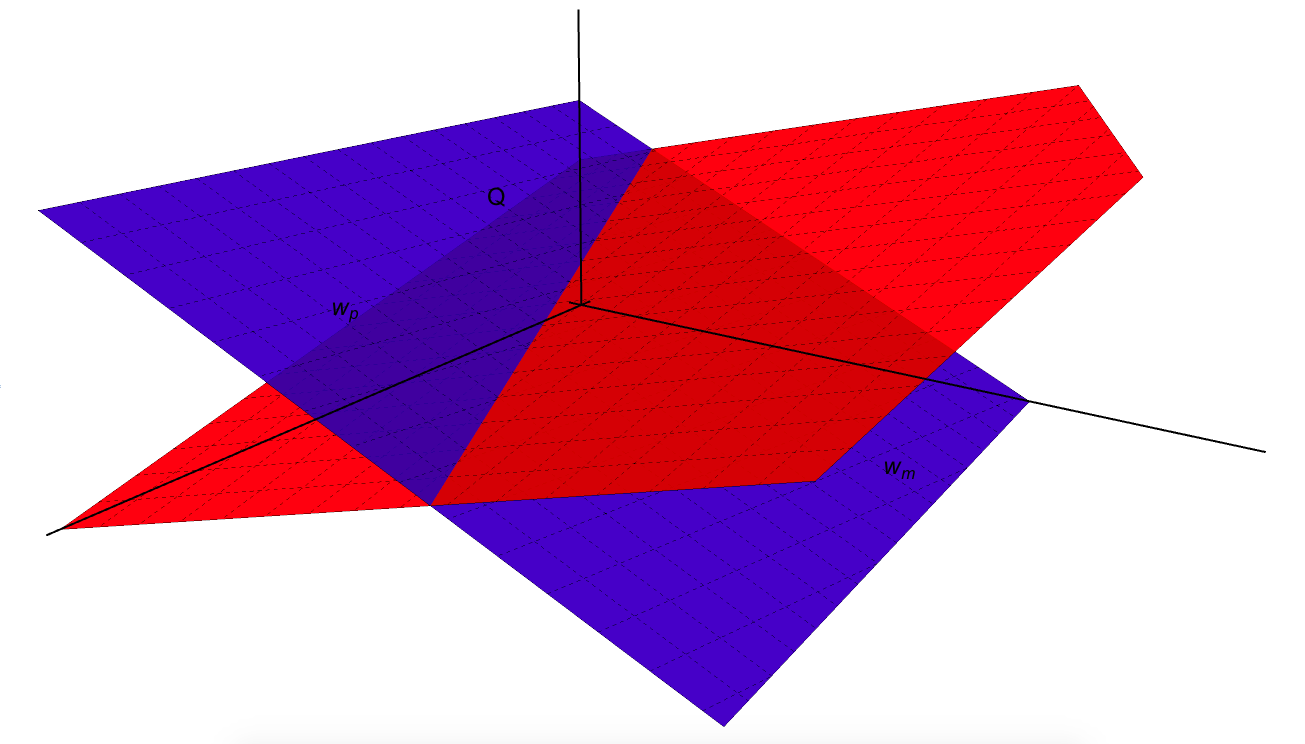
\includegraphics[scale=0.3]{qgraphfull.png}
    \caption{Plot of the quantity $Q$ of M-types and P-types demanded vs. $w_m$ and $w_p$. Here, the blue plane is the quantity of M-types demanded by the firm, and the red plane is the number of P-types demanded. These planes add to the total number of people hired by the firm. Note, later the ``poetry premium" is discussed. Here, this is just represented as a vertical slice out of the graph.}
\end{figure}

\begin{figure}
    \centering
    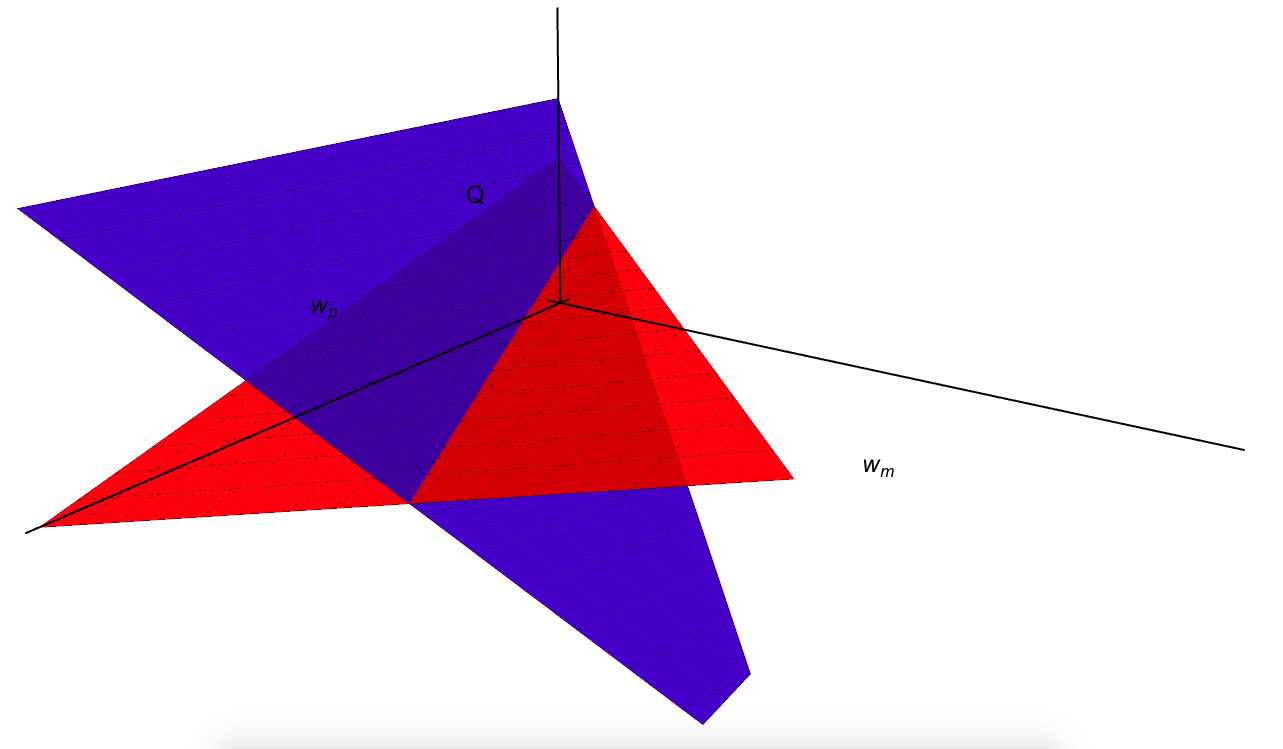
\includegraphics[scale=0.3]{qgraphhalf.png}
    \caption{Shown here is a restriction of the graph above to half of the first quadrant, where $w_p > w_m$.  Note: these graphs do not tell us anything about the \textit{equilibrium} quantities - they are simply demand functions.}
\end{figure}



Recall that individuals maximize based on a two-period utility function where they spend all the money they receive in a given period. Their parents give them $y$ units of currency as they exit high school. The labor supply function is a step-function where people all people will become P-types if
\[
    u(y - kT_1) + \beta{}u(w_pT_2) > u(y + w_mT_1) + \beta{}u(w_mT_2).
\]
They will become M-types if the inequality is reversed. The labor supply curve is vertical where the two expressions are equal. Suppose that $u(m) = m$. Then the equality case becomes
\[
    w_p = (w_m + k)\frac{T_1}{T_2} + w_m.
\]


Assume that the wage for M-types is above the reservation wage so that everyone is employed. We will use a different production function to make $NL_p$ well-defined in terms of the poetry premium:
\[
    f(L_m, L_p) = C_m\log(L_m + L_p) + C_p\log{L_p}.
\]
By our first-order condition from Problem 1,
\[
    \frac{C_m}{L_m + L_p} = w_m \text{ and } \frac{C_m}{L_m + L_p} + \frac{C_p}{L_p} = w_p.
\]
Rearranging gives us
\[
    L_m + L_p = \frac{C_m}{w_m} \text{ and } L_p = \frac{C_p}{w_p - w_m}
\]
If the total population is $L$, we have the extra condition that $NL_m + NL_p = L$, and so the number of P-types $NL_p$ demanded is
\[
    \frac{LL_p}{L_m + L_p} = L_p = \frac{C_pL}{C_m(w - 1)},
\]
where $w = w_p/w_m$ is the wage premium (note, by the last problem, as long as the cost of college is positive $w_p > w_m$, so this function is well defined on its domain).

As for the labor supply, it suffices to write the equality case
\[
    w_p = (w_m + k)\frac{T_1}{T_2} + w_m
\]
in terms of $w$. Let the annual tuition $k$ depend on $w_p$ so that $k = k_pw_p$. There are two motivations for this. First, we want the tuition to scale up with inflation. Second, we want the wage obtained as a P-type to increase with the cost it takes to become one. (Secretly, these are the same reason.) Dividing through by $w_m$ gives us
\[
    w = (1 + k_p)\frac{T_1}{T_2} + 1.
\]

Using this, we can make a plot of the labor supply and demand as a function of the number of P-types and the poetry premium.  This is shown in Figure 3.  Note, you might be wondering what happens in equilibrium if the demand curve happens to go in between the steps in the supply function.  In our model, this situation is a singularity in our model.  However, it can be easily addressed.  In reality, the supply function will be more smooth than it is here: the places in between the steps of the supply function will be filled in, due to slight preference differences in the labor choice of people.  The cutoff for some people will be slightly different than others, and as a result, there will always be a point where the demand intersects the supply.

\begin{figure}
    \centering
    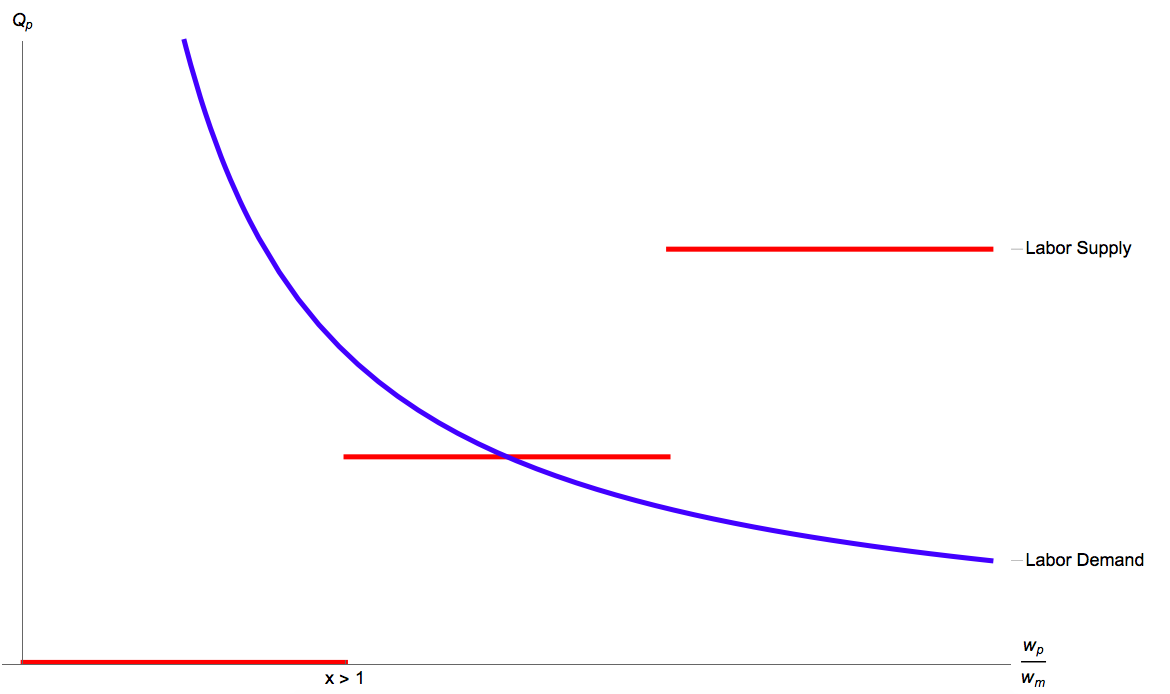
\includegraphics[scale=0.35]{qpvsratio.png}
    \caption{Shown here is the labor demand and supply with the quantity of P-types, $Q_p$, on the y-axis, and the wage premium, $\frac{w_p}{w_m}$, on the x-axis.}
\end{figure}

An increase in real tuition corresponds to an increase in $k_p$ in our model. This means that the poetry premium $w$ increases because it will take more money to continue convincing people to become P-types. This is evident from the labor supply condition
\[
    w = (1 + k_p)\frac{T_1}{T_2} + 1.
\]
An increase in $w$ decreases the number of P-types in equilibrium because firms are not as willing to pay for P-types as before. This is evident from the labor demand condition
\[
    NL_p = \frac{C_pL}{C_m(w - 1)}.
\]

	\item{The Government of Skillistan wants society to have more P-types than it currently
does and decides to subsidize the tuition fee at Skillvard College.}

\begin{enumerate}

	\item{Does this subsidy increase the number of P-types in society?}
	\item{What are the aggregate consequences of this subsidy for residents and firms? In
other words, who benefits from the subsidy?}
	\item{The Government is also a player in this economy. It cares most about the welfare
of residents, somewhat less about its own welfare and the least about the
welfare of firms. Is the fee subsidy a Pareto improvement over the status quo?
If not, suggest an alternative policy that would be a Pareto improvement.}

\end{enumerate}

\section*{Part 4}

Suppose that the government decides to subsidize the price of college.  This will have two effects: first, more people will go to college, because it is cheaper, and second, the increase in the number of people going to college will cause wages for P-types to go down, which will cause people to be less likely to become P-types.  Using the Slutsky equation, we see that by a mild abuse of notation, the net effect of a change in the price of college can be captured by 
$$
\dfrac{dQ_p}{dk} = \qpartial{Q_p}{k} - \qpartial{Q_p}{D}(Q_p)
$$

Thus, we see that the number of P-types will increase if the demand is relatively inelastic, and vice-versa.  From the third part of the model, we see that that the demand will almost certainly be elastic enough so that this holds.  Equivalently, we can check this by examining our condition from the second part of the model:

$$
u(y - k T_1) + \beta u(w_p T_2) = u(y + w_m T_1) + \beta u(w_m T_2)
$$

This fits in to the first part of the Slutsky equation - it shows that people will clearly be incentivized to go to college because of the decrease in price, holding demand constant.  However, in the case of a general demand function, the total change in the number of P-types.  For example, the firm could have a production function that requires exactly a specific number of P-types without which it cannot produce.  In this case, there will be times when subsidizing college will do nothing to the total number of P-types.  However, using our demand function

$$
L_p = \frac{C_p L}{C_m(w - 1)}
$$

from the second part, we see that the outcome is likely to be positive.  That is, subsidizing college will increase the total number o P-types in society.  

We see therefore that an subsidy of the college tuition will change the value of "$x$" in the demand and supply in the graph above - that is, it will make the cutoff lower for the point when people decide to go to college.  Of course, the value it shifts to must still be greater than 1, since people will still not go to college if they can make more money working as an M-type anyway (unless the government pays people more than $w_m$ to go to college - but we assume that the government isn't that rich).  Suppose this shifts the value of $x$ to a value $1 < y < x$.  The graphs are represented in Figure 4 and 5.  If it is true that the government wanted more P-types, then we could assume that there was some initial deadweight loss due to a social externality.  This is the gray area.  We thus see that the subsidy benefits the workers.  However, if the government was wrong, and there were not in fact too many P-types to begin with, then this subsidy will hurt the workers. 



Now, since the government does not really care about the firm, and it cares somewhat about itself, we see that this is not a Pareto improvement - the government is providing money as a subsidy, and is thus less well off, since the subsidy causes no additional tax revenue.  If the government wanted a Pareto improvement over the current state, it could tax the firm.  Since the labor supply function is horizontal, a tax on the firm will not cause a decrease in the surplus of the workers.  However, if the government taxes the firm, it will generate additional revenue for itself, leaving the citizens' welfare unchanged.  Thus, it has improved its own state without causing a decrease in the state of anyone else.  The firm is possibly harmed by this action, but the goernment does not care about the firms, so this is a Pareto improvement.  (Note, Figure 4 and Figure 5 are on the next page.)

\begin{figure}[b]
    \centering
    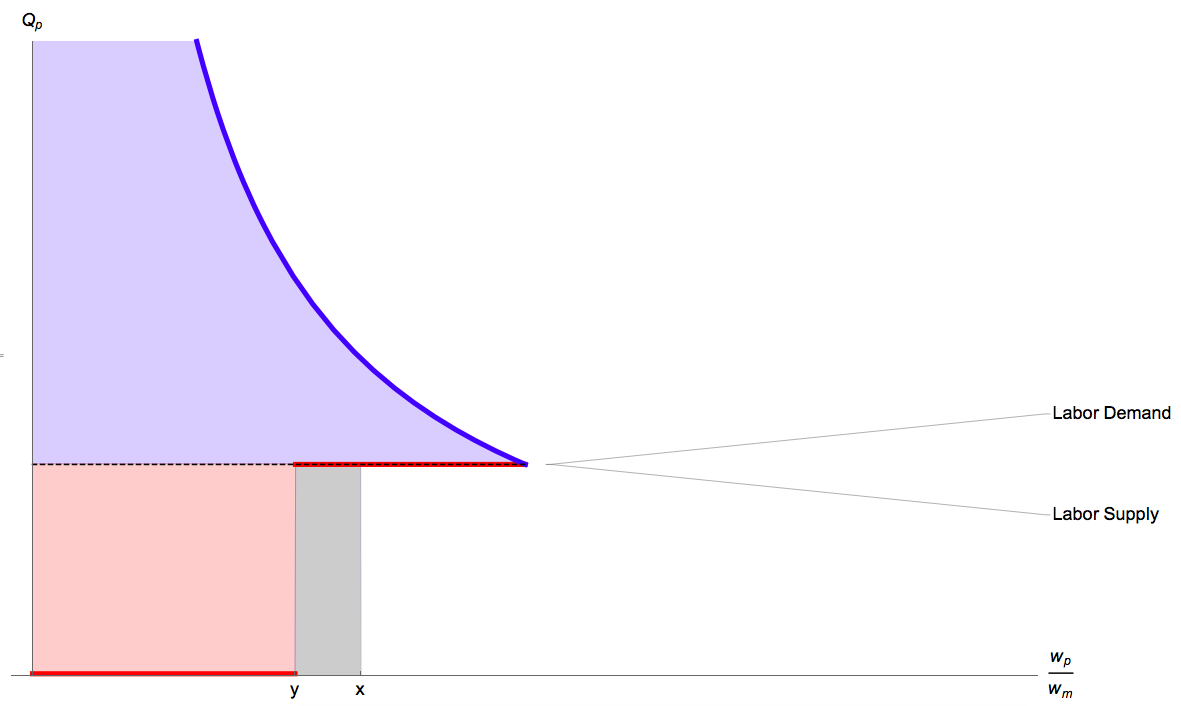
\includegraphics[scale=0.25]{withloss.png}
    \caption{Here, we see that there is an initial deadweight loss in the system due to having too few P-types in society.  This deadweight loss is represented in gray.  The optimal ratio of P-types to M-types is $y < x$.}
\end{figure}

\begin{figure}[b]
    \centering
    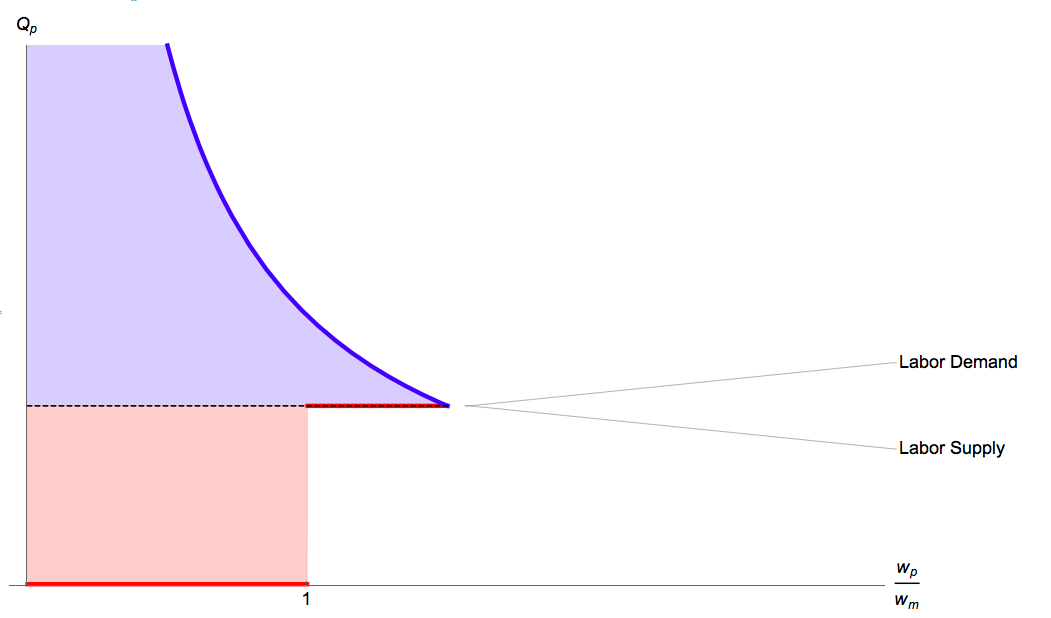
\includegraphics[scale=0.3]{noloss.png}
    \caption{This shows the surplus after the government action, with the deadweight loss gone.  However, if the government was wrong, then this would in fact create more deadweight loss.}
\end{figure}




\end{enumerate}
\end{document}
